\documentclass[tikz]{standalone}

\usepackage{tikz}
\usetikzlibrary{positioning,shapes,backgrounds}
\usepackage{tkz-euclide}

\begin{document}

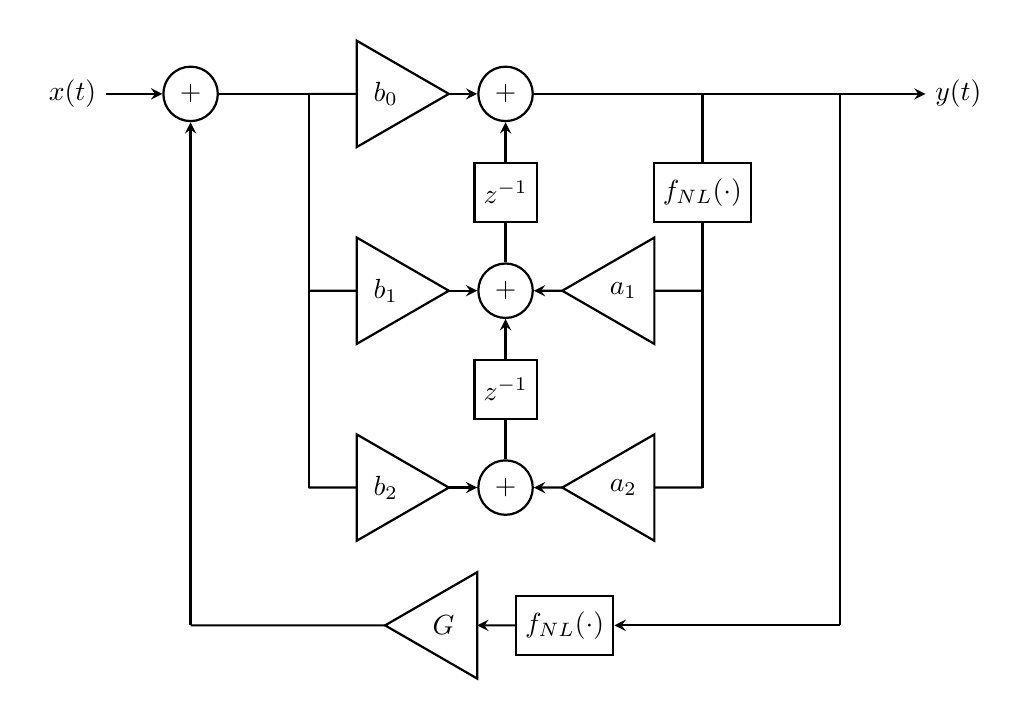
\begin{tikzpicture}[node distance=1.5cm, background rectangle/.style={fill=white}, show background rectangle]
    \tikzset{
        mynode/.style = {rectangle, line width=0.8pt, minimum width=1.0cm, minimum height=0.75cm, text centered, draw=black, fill=white},
        amp/.style = {regular polygon, regular polygon sides=3, draw, fill=white, text width=1em,
                      inner sep=1mm, outer sep=0mm, shape border rotate=-90, line width=0.8pt},
        arrow/.style = {thick,->,>=stealth},
        delay/.style = {rectangle, draw=black, line width=0.8pt, minimum height=0.75cm}
    }
    \node (input) {$x(t)$};
    \node (sum) [draw, fill=white, circle, line width=0.8pt, right of=input] {+};
    \draw [arrow] (input) -- (sum);
    
    \coordinate[right of=sum] (splitb0);
    \coordinate[below of=splitb0, yshift=-1.0cm] (splitb1);
    \coordinate[below of=splitb1, yshift=-1.0cm] (splitb2);
    \draw [thick] (sum) -- (splitb0);
    \draw [thick] (splitb0) -- (splitb1);
    \draw [thick] (splitb1) -- (splitb2);

    \node[amp, right of=splitb0, xshift=-0.5cm] (b0) {$b_0$};
    \node[amp, right of=splitb1, xshift=-0.5cm] (b1) {$b_1$};
    \node[amp, right of=splitb2, xshift=-0.5cm] (b2) {$b_2$};
    \draw [thick] (splitb0) -- (b0);
    \draw [thick] (splitb1) -- (b1);
    \draw [thick] (splitb2) -- (b2);

    \node (sum0) [draw, fill=white, circle, line width=0.8pt, right of=b0] {+};
    \node (sum1) [draw, fill=white, circle, line width=0.8pt, right of=b1] {+};
    \node (sum2) [draw, fill=white, circle, line width=0.8pt, right of=b2] {+};
    \draw [arrow] (b0) -- (sum0);
    \draw [arrow] (b1) -- (sum1);
    \draw [arrow] (b2) -- (sum2);

    \node (z1) [delay, below of=sum0, yshift=0.25cm] {$z^{-1}$};
    \node (z2) [delay, below of=sum1, yshift=0.25cm] {$z^{-1}$};
    \draw [thick] (sum1) -- (z1);
    \draw [thick] (sum2) -- (z2);
    \draw [arrow] (z1) -- (sum0);
    \draw [arrow] (z2) -- (sum1);

    \coordinate[right of=sum0, xshift=1.0cm] (splita0);
    \node (NL) [mynode, below of=splita0, yshift=0.25cm] {$f_{NL}(\cdot)$};
    \coordinate[below of=splita0, yshift=-1.0cm] (splita1);
    \coordinate[below of=splita1, yshift=-1.0cm] (splita2);
    \draw [thick] (sum0) -- (splita0);
    \draw [thick] (splita0) -- (NL);
    \draw [thick] (NL) -- (splita1);
    \draw [thick] (splita1) -- (splita2);

    \node[amp, left of=splita1, shape border rotate=90, xshift=0.5cm] (a1) {$a_1$};
    \node[amp, left of=splita2, shape border rotate=90, xshift=0.5cm] (a2) {$a_2$};
    \draw [thick] (splita1) -- (a1);
    \draw [thick] (splita2) -- (a2);
    \draw [arrow] (a1) -- (sum1);
    \draw [arrow] (a2) -- (sum2);

    \coordinate[right of=splita0, xshift=0.25cm] (split);
    \node (output) [right of=split] {$y(t)$};
    \draw [thick] (splita0) -- (split);
    \draw [arrow] (split) -- (output);

    \coordinate[below of=split, yshift=-5.25cm] (low_right);
    \node (NL) [mynode, left of=low_right, xshift=-2.0cm] {$f_{NL}(\cdot)$};
    \node (G) [amp, left of=NL, shape border rotate=90] {$G$};
    \coordinate[below of=sum, yshift=-5.25cm] (low_left);


    \draw [thick] (split) -- (low_right);
    \draw [arrow] (low_right) -- (NL);
    \draw [arrow] (NL) -- (G);
    \draw [thick] (G) -- (low_left);
    \draw [arrow] (low_left) -- (sum);
\end{tikzpicture}

\end{document}
